\documentclass[border=1mm]{standalone}

\usepackage{listings}
\usepackage{tikz}

\usetikzlibrary{decorations.pathreplacing,calligraphy}

\begin{document}

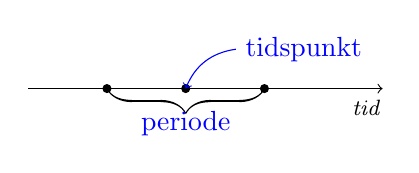
\begin{tikzpicture}[decoration={calligraphic brace, amplitude=9pt}]
   \draw [->] (-1,0) -- (3.5,0);
 \foreach \Point/\PointLabel in {(0,0)/a_1, (1,0)/b, (2,0)/a_2}
        \draw[fill=black] \Point circle (0.05) node[above] {};
   \node (pt) at (2.5,0.5) {\textcolor{blue}{tidspunkt}} ;
   \path [->,draw,blue] (pt.west) to [bend right] (1,0) ;
 %% \foreach \Point/\PointLabel in {(0,0)/a_1, (1.5707,0)/b_2, (0.7853,0)/a_2}
        %% \draw[fill=black] \Point circle (0.05) node[below] {$\PointLabel$};
 %% \draw[decorate,thick] (0,-0.8) -- node[below=1ex](I0){$I_0$} (3.1415,-0.8);
 %% \draw[decorate,thick] (0,-0.4) -- node[below=1ex]{$I_1$} (1.5707,-0.4);
   \draw[decorate,thick] (2,0) -- node[below=1ex]{\textcolor{blue}{periode}} (0,0);
   \node at (3.3,0) [yshift=-1.6ex] {\emph{\footnotesize tid}} ;
\end{tikzpicture}

\end{document}
